\documentclass[french]{rapportENSTAB}
\usepackage{lipsum}
\usepackage{graphicx}
\usepackage{float}
\usepackage{subfloat}
\usepackage{caption}
\usepackage[utf8]{inputenc}
\usepackage[T1]{fontenc}
\usepackage{babel}
\usepackage{enumitem}
\usepackage{tabularx}
\usepackage{titlesec}
\usepackage{multicol,caption}
\usepackage[colorlinks=true,linkcolor = red, breaklinks]{hyperref}
\hypersetup{
    colorlinks=true,
    linkcolor= gray,
    urlcolor=blue,
}
\usepackage{textcomp}
\usepackage{appendix}


\title{PAi} %Titre du fichier

\begin{document}

%----------- Informations du rapport ---------

\titre{Rapport de Projet Industriel } %Titre du fichier .pdf
\UE{UE 4.4} %Nom de la UE

\eleves{Ludovic \textsc{diguet}\\Antonin \textsc{lizé}\\Maha \textsc{halimi}\\Badr \textsc{moutalib}}%Nom des élèves


\commanditaire{\textsc{orange} Labs\\Jacques \textsc{Chodorowski} \\  \bigskip \\ \bigskip}

%----------- Initialisation -------------------
        
\fairemarges %Afficher les marges
\fairepagedegarde %Créer la page de garde
\tableofcontents
\newpage
%------------ Corps du rapport ----------------

\section{Introduction} 
\subsection{Présentation générale} 
Notre projet a pour objectif de construire un robot patrouilleur pour explorer une ferme de routeurs, ceci afin de prendre des vidéos et photos des serveurs et ainsi permettre à distance un premier diagnostic des problèmes rencontrés dans le centre de serveurs. Les fonctions principales de ce robot ont été définies ci-dessous :\begin{itemize}[label=\textbullet, font=\small\color{blue}]
    \item Être capable de patrouiller dans une zone présentant des obstacles (murs, câbles au sol…).
    \item Pouvoir prendre des vidéos et des photos exploitables.
    \item Être capable de retourner de manière autonome à sa station de recharge.
    \item Communiquer les informations acquises.
    \item Être intégrable sous ROS.
\end{itemize}\\


Pour bien comprendre tous les enjeux de ce projet nous avons eu besoin d’effectuer plusieurs conférences téléphoniques avec Mr CHODOROWSKI qui ont donné lieu à plusieurs rencontres à l’ENSTA afin d’aborder de façon plus détaillée certains points. Ces rencontres nous ont permis de bien définir le projet dans sa globalité et ainsi pouvoir réaliser un cahier des charges fonctionnel que ce soit pour le robot ou pour la station de recharge.\\

Vous pouvez également retrouver notre projet sur \href{https://github.com/AntoninLize/Projet_OrangeLabs}{GitHub}. Tous les codes Arduino et C++ se trouvent dessus, les liens qui renvoient vers notre code dans la suite du projet pointent tous vers notre GitHub. \\

\textit{A noter que tous les mots colorés sont des liens à suivre qui permettent de se diriger vers un site internet ou vers une autre partie du rapport}.
\\


\subsection{Abstract}

Ce rapport traite du projet en collaboration avec Orange Labs pour la création d’un robot terrestre  autonome. Le produit abouti visé est un véhicule capable de naviguer dans des salles de serveurs de manière autonome afin d’y identifier une éventuelle panne. Ce rapport traite du cheminement suivi. 
Après avoir dressé le cahier des charges du robot en collaboration avec notre encadrant, nous avons fixé deux objectifs majeurs pour ce projet : la construction d’un drone terrestre fonctionnel et la construction de la station de recharge pour ce drone. \\

Certaines contraintes nous ont poussés à redéfinir nos objectifs : nous sommes arrivés à deux résultats majeurs. Premièrement une description théorique de la manière de construire le robot et la station de recharge. Deuxièmement l’ensemble des composants sont intégrés et prêts à être utilisés sous ROS. Ces résultats sont satisfaisants et permettront d’assurer la continuité du projet. \\

Ce projet est une opportunité pour nous d’appliquer les connaissances acquises dans de nombreux domaines mais aussi de travailler avec des outils nouveaux pour nous, comme notamment l’utilisation d’un NUC et d’un LIDAR. De plus, la collaboration avec l’entreprise ORANGE LABS fut une occasion de réellement progresser en matière de gestion de projet et de définition d’objectifs.
\\

\subsection{Remerciements}
La réalisation de ce projet a été possible grâce au concours de plusieurs personnes à qui nous voudrions témoigner toute notre gratitude.\\ 

Nous tenions à exprimer toute notre reconnaissance à notre professeur référant, Monsieur Fabrice LEBARS. Nous le remercions de nous avoir encadrés, orientés, aidés et conseillés.\\

Nous adressons nos sincères remerciements à tous les professeurs, intervenants et toutes les personnes qui par leurs paroles, leurs écrits, leurs conseils et leurs critiques ont guidé nos réflexions et ont accepté de nous rencontrer et de répondre à nos questions durant nos recherches.\\

Enfin nous voulions remercier tout particulièrement notre encadrant Mr Jacques\\
CHODOROWSKI d’Orange Labs à Lannion pour son aide et sa supervision tout au long du projet. Il nous a permis de toujours garder en ligne de mire des objectifs clairs et il a su adapter les modalités du projet au vu du contexte actuel et des contraintes imposées par celui-ci. Ce fut un réel plaisir pour toute notre équipe de travailler en collaboration avec lui. \\

À tous ces intervenants, nous présentons nos remerciements, notre respect et notre gratitude.\\

\pagebreak
\section{Définition du problème global}
\subsection{Partie Station de Recharge}
Dans cette sous partie, nous allons énumérer les contraintes qui nous permettront d'élaborer et de choisir des solutions pour la réalisation de la Station de recharge. \\

Voici donc le Cahier des Charges fonctionnel pour la partie Station de Recharge:

\begin{figure}[H]
    \centering
    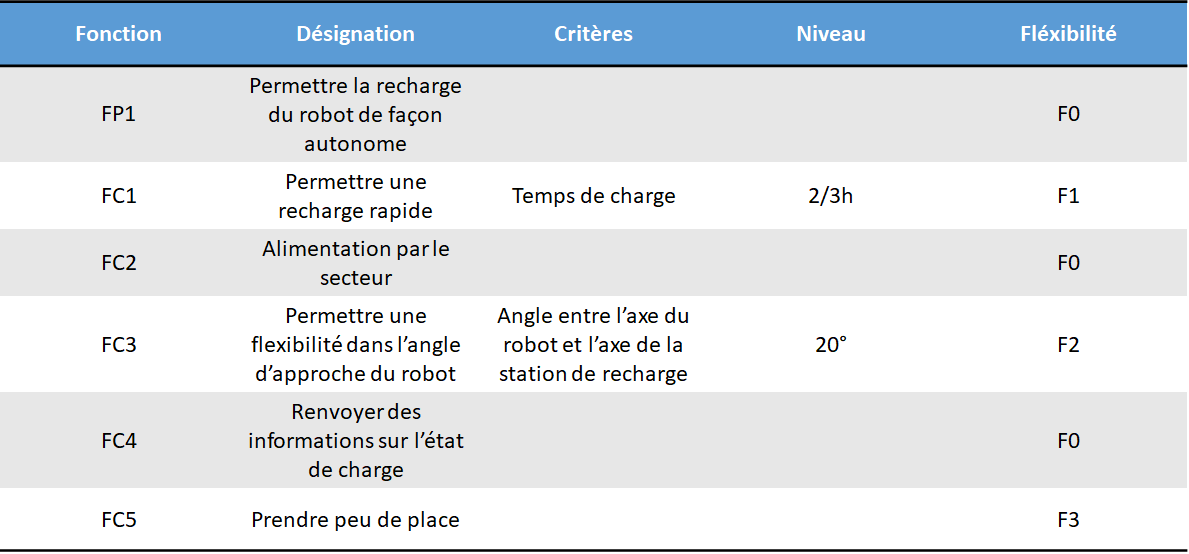
\includegraphics[scale=0.65]{images/station de recharge/Cahier des Charges station.png}
    \caption{Cahier des Charges Fonctionnel - station de recharge}
    \label{fig:cdcf}
\end{figure}

Ces Cahiers des Charges, ont étés élaborés à partir de nos rencontres avec Monsieur \textsc{chodorowski} et nous ont permis de définir les principaux axes de travail pour la suite. Un document qui nous a également servi pour définir les contraintes et les enjeux se trouve sur le  \href{https://github.com/AntoninLize/Projet_OrangeLabs}{GitHub} du projet et se nomme "\textit{OrangeLabs - Robot autonome évolutif}".\\

Les grands axes sont donnés dans la Figure ci-dessus, et ce sont ces axes qui nous ont dicté nos choix que ce soit pour les choix des composants, ou les choix de l'architecture et de la forme de la Station de Recharge. Nous reviendrons dans \hyperlink{partie_station2recharge}{la partie dédiée à la conception de la Station de Recharge}, sur les différentes contraintes clés.\\


Il est important de noter que ces cahiers des charges sont ceux de la version finale robot. Les objectifs de notre travail sont plus concentrés sur certaines parties que d'autres et ont évolué au cours du projet et face aux difficultés rencontrées, le  détail de l'évolution de nos objectifs est abordé dans la sous-section suivante. \\ 

\subsection{Partie robot}

L'objectif général du projet est de construire un robot terrestre capable de naviguer en intérieur de manière totalement autonome. Il doit également être capable d'évoluer sur un terrain plus ou moins accidenté pour s'adapter à l'organisation de certains data center où les obstacles sont nombreux. Avec notre encadrant, il a été défini que le robot devrait pouvoir évoluer dans des couloirs d'environ 60 cm de largeur. En plus de sa capacité à patrouiller de manière indépendante, le robot doit également être capable de se recharger sans intervention extérieure. La contrainte de vitesse de déplacement,  fixée par l'encadrant du projet, est d'un mètre par seconde. \\

En plus de sa capacité à naviguer de manière totalement autonome, il faut également qu'un technicien puisse contrôler le robot si nécessaire. Il faudra donc prévoir une commande manuelle et un bouton d'arrêt d'urgence en cas de problème. \\

Venons en maintenant à la partie échange d'information. La première contrainte importante, exigée par notre encadrant, est l'utilisation du middleware ROS afin de faciliter l'intégration des composants et d'organiser le projet. Le robot doit pouvoir échanger des informations avec l'utilisateur, notamment par un retour vidéo qui permettrait au technicien d'identifier une éventuelle panne. Cette caméra serait dans l'idée, fixée sur un mat d'environ 1.80 m (sur lequel d'autres composants pourraient être ajoutés si nécessaire).\\

C'est à partir de l'ensemble de ces contraintes nous avons élaboré le cahier des charges ci-dessous. \\


\begin{figure}[H]
    \centering
    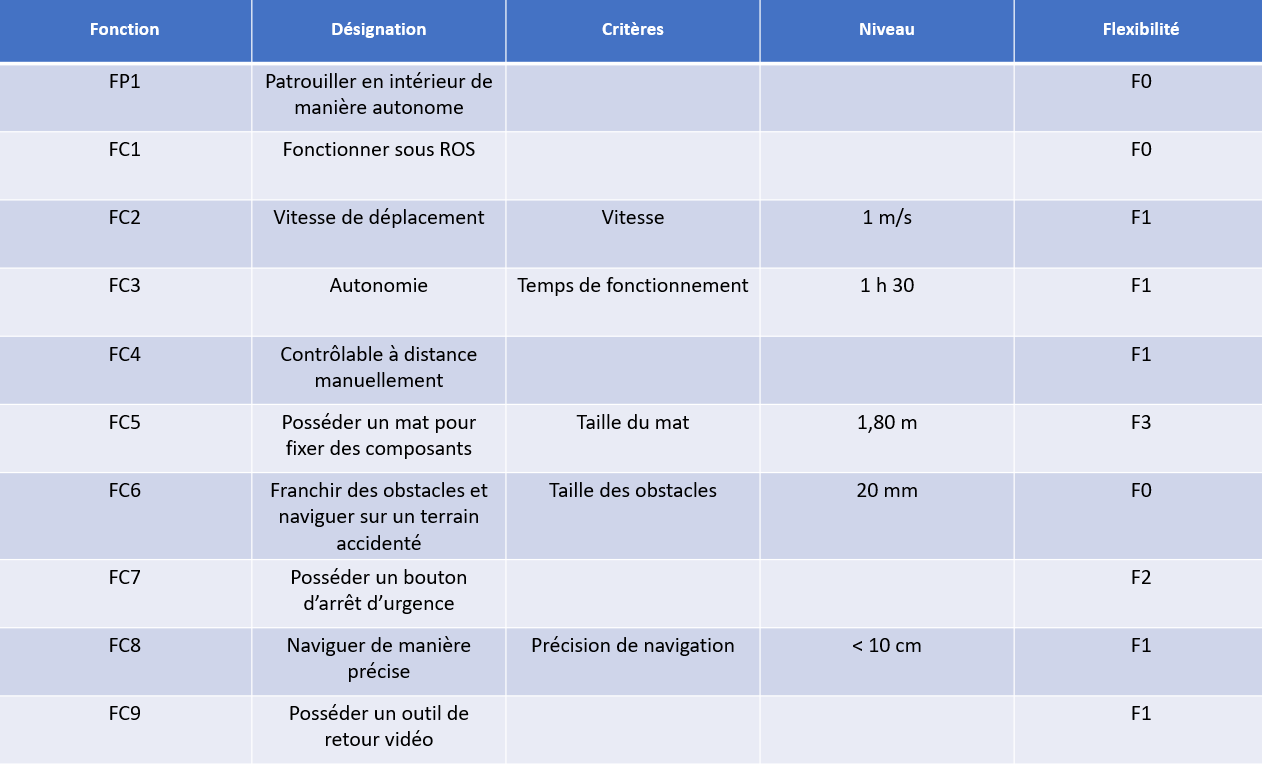
\includegraphics[scale=0.5]{images/robot/cahier_charge_robot.png}
    \caption{Cahier des Charges Fonctionnel - Robot}
    \label{fig:cdcf}
\end{figure}


\subsection{Définition et évolution des objectifs au cours du projet}

La réalisation du robot présenté ci-dessus en partant de zéro est très ambitieuse par rapport au temps alloué au projet : il a donc été convenu que l'objectif principal serait la construction "hardware" du robot, la partie algorithme pouvant être fournie par notre encadrant en utilisant des projets similaires déjà développés. Le but de notre projet au long de l'année est donc la construction du robot pour arriver à un produit  fonctionnel et contrôlable manuellement. Les enjeux se résument de la manière suivante :  \begin{itemize}[label=\textbullet, font=\small\color{blue}]
    \item Construire un robot fonctionnel sur lequel pourrait être intégré un algorithme de navigation autonome et respectant les contraintes du cahier des charges.
    \item Construire une station de recharge pour ce robot.
\end{itemize}   \\ 


Cet objectif était réalisable dans le temps imparti, cependant entre la perte de deux personnes travaillant sur le projet (pour cause de départ en substitution en janvier) et la  difficulté majeure liée à la crise du COVID-19, nous avons dû redéfinir nos objectifs. Au moment du confinement il était impossible d'avoir accès à la totalité des composants du robot, donc, en plus de ce qui était déjà réalisé, nous avons décidé que l'objectif du projet serait, à défaut de pouvoir construire le robot, de réaliser un travail théorique le plus précis possible, détaillant le processus de construction et d'intégration, ainsi que les choix techniques. Ce travail permet de constituer une base de travail intéressante pour la suite du projet et permet d'en assurer la continuité.

\section{Choix techniques pour le Robot}
\subsection{Architecture globale}

Le cahier des charges nous permet d'identifier les différentes fonctions que notre robot doit être capable de réaliser, il nous faut intégrer : 
 \begin{itemize}[label=\textbullet, font=\small\color{blue}]
    \item Un support pour le robot.
    \item Un moyen de propulsion approprié.
    \item Des capteurs pour l'acquisition des informations nécessaires.
    \item Des moyens d'alimentation adéquats.
    \item Des outils de contrôle et d'interface.
\end{itemize}   \\ 

L'organisation de ces composants choisis  est détallée dans le schéma ci-dessous. Le détail des choix pour chaque composant sera donné dans une partie ultérieure.

 \\
 
 \begin{figure}[H]
    \centering
    \includegraphics[scale=0.43]{images/robot/schéma_info_2_png.png}
    \caption{Organisation des composants - Architecture générale}
    \label{fig:cdcf}
\end{figure}

\\

Il est également important de préciser le mode de communication choisi entre ces différents composants, voir ci-dessous.

\\

 
 \begin{figure}[H]
    \centering
    \includegraphics[scale=0.46]{images/robot/schéma_info_png.png}
    \caption{Organisation des composants - Modes de communication}
    \label{fig:cdcf}
\end{figure}

\\

\subsection{Partie Mécanique : le châssis}
Très vite nous avons compris que le choix du châssis allait être primordial pour la suite du projet et surtout qu'il devait être effectué assez rapidement. En effet en fonction du châssis choisi, les choix tels que ceux des moteurs, des composants électroniques et des capteurs allaient être impactés. Après discussion avec notre encadrant, deux choix apparaissaient : \begin{itemize}[label=\textbullet, font=\small\color{blue}]
    \item Le premier était de construire nous-mêmes un châssis en le modélisant sur \textit{Autodesk Inventor} et ensuite d'acheter les batteries, les roues et les moteurs;
    \item Le second était d'utiliser un châssis tout fait avec les roues et les emplacements moteurs.
\end{itemize}\\

L’avantage du premier choix était que nous pouvions totalement designer le robot comme nous le souhaitions. Mais l’inconvénient se trouvait au niveau de la robustesse du robot notamment si nous utilisions un système de chenilles. \\

Pour le second, l'avantage était que nous n’avions pas besoin de tenir compte des problèmes de robustesse cependant les dimensions n'étaient pas modulables à notre convenance. \\

Avant de choisir nous avions tenté de modéliser un robot imprimable en 3D ou usinable avec les outils disponibles à l'\textit{ENSTA Bretagne}. En voici quelques photos :

\begin{figure}[H]
    \centering
    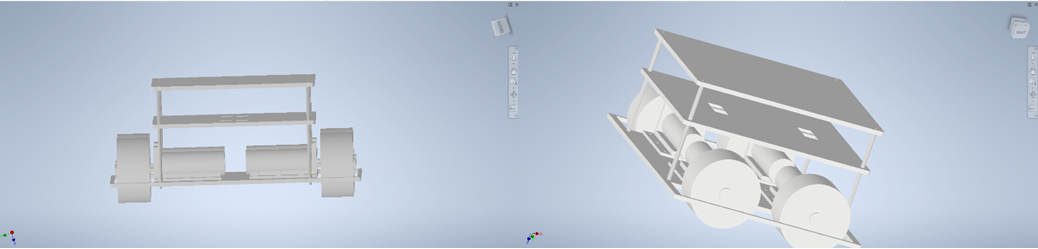
\includegraphics[scale=0.70]{images/robot/chassis 3D.png}
    \caption{Modélisation 3D du robot}
    \label{fig:cdcf}
\end{figure}

Finalement nous avons opté pour la solution du châssis à acheter sur internet pour des raisons de précision au niveau des roues (pour notre modélisation) ou des chenilles (pour le choix final). Notre encadrant préférait également un robot construit à partir de composants sur étagères ou achetés chez des fournisseurs de son entreprise.  \\

Nous avons donc dû faire la prospection des châssis vendus sur internet en faisant attention à la fois au prix, aux options d’achats (moteur inclus ou non) mais surtout aux dimensions et à la possibilité d’ajouter nos composants facilement.\\ 

Le choix final s’est donc porté sur un châssis robuste et qui rendait l'ajout d'étages possible simplement. Voici l’agent 390 que nous avons décidé de prendre sur \textit{RobotShop} par rapport aux options utiles : 

\begin{figure}[H]
    \centering
    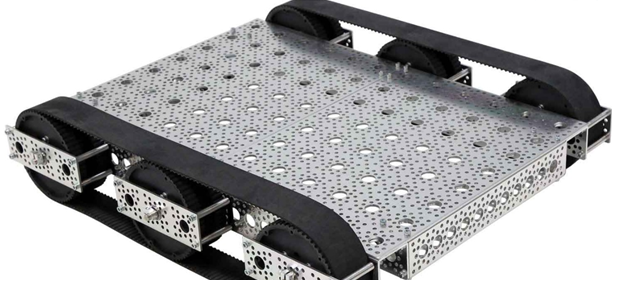
\includegraphics[scale=0.70]{images/robot/chassis.png}
    \caption{Châssis Robotique Agent 390}
    \label{fig:cdcf}
\end{figure}\\
\href{https://www.robotshop.com/eu/fr/kit-robot-chenilles-agent-390-avec-moteurs.html}{Lien du site pour le châssis avec ses  caractéristiques.}\\

Ce châssis respectait les dimensions préconisées dans le Cahier des Charges et il permettait de ne pas prendre ces moteurs et donc de pouvoir en choisir avec un couple suffisant. Nous allons d'ailleurs maintenant parler du choix des moteurs.\\


\subsection{Partie Électronique}
\subsubsection{Choix des moteurs}
Le choix des moteurs a été relativement simple. Nous avons cherché à garder la même taille de moteur que ceux qui pouvaient être vendus avec le châssis. Cependant nous avons cherché un moteur avec des encodeurs et possédant un couple plus important et une vitesse de rotation qui soit proche . \\

Le couple nécessaire a été calculé par Monsieur \textit{Thierry ROPERT} (professeur de mécanique) en prenant en compte le diamètre des roues, la pente maximale à franchir et le poids (frottement pas pris en compte). Nous sommes arrivés à la conclusion qu'un couple de 2 N.m était nécessaire.\\

Le robot devant avancer à une vitesse de 1m/s, nous avons dû calculer avec le diamètre des roues la vitesse nominale du moteur. Le résultat donne environ \textit{200 RPM}.\\

Sur la base de nos besoins nous avons donc décidé de choisir le moteur suivant : 

\begin{figure}[H]
    \centering
    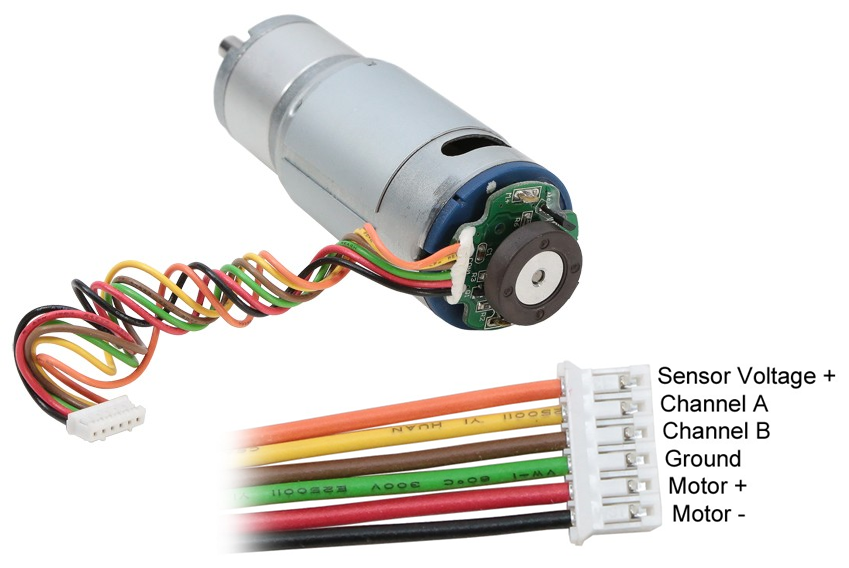
\includegraphics[scale=0.70]{images/robot/moteur.png}
    \caption{Choix du moteur}
    \label{fig:cdcf}
\end{figure}\\ 
\href{https://www.servocity.com/313-rpm-hd-premium-planetary-gear-motor-w-encoder}{Lien site moteur avec caractéristiques}.\\

\subsubsection{Choix capteurs}

Les choix qui doivent être fait pour les capteurs sont, la caméra, le LIDAR, et les encodeurs. \\
La caméra a été fournie par notre encadrant, c'est une caméra Realsense T265. Cette caméra est très précise et elle est bien adaptée pour l'optométrie visuelle. Sa facilité d'intégration avec ROS en fait également un excellent choix.\\
Le choix du LIDAR a été fait grâce aux conseils de Monsieur \textbf{Fabrice LEBARS}. Le choix final est un RPLIDAR A2 de chez Slamteck. Il est approprié pour la détection d'obstacle en intérieur à des distances correspondant aux attendus.\\
Les encodeurs sont choisis par rapport au moteur, ils sont livrés avec.




\subsubsection{Choix des batteries}
Afin de permettre l'alimentation de tous nos composants électroniques, nous avons dû choisir une batterie. Tout d'abord de notre propre initiative nous avons décidé de séparer l'alimentation \textit{\textbf{Moteur + Arduino UNO + Motor Shield}} de l'alimentation \textit{\textbf{NUC + Autres Capteurs}}. En effet comme nous avions vu en cours, cela permet d'éviter la sous-alimentation de certains capteurs ou contrôleurs dans le cas où les moteurs auraient besoin d'un pic de courant.\\
Nous avons également dû tenir compte du Cahier des Charges du robot, qui stipule environ 1h30 d'autonomie.

\\

 \begin{figure}[H]
    \centering
    \includegraphics[scale=0.6]{images/robot/schéma_elec_png.png}
    \caption{Architecture électronique obtenue}
    \label{fig:cdcf}
\end{figure}


Il est à noter que les batteries que nous possédons actuellement ne sont pas les plus appropriées puisqu'il a fallu en brancher deux en série pour obtenir l'intensité adéquat. Après une étude de la puissance nécessaire au fonctionnement des composants il a été convenu que le choix le plus approprié serait une batterie LiPo 160000 mah (voir  \href{https://www.iplanes-rc.fr/produit/batterie-lipo-22-2-volt-16000mah-25c/}{ici}).
Il convient simplement de remplacer dans le schéma ci-dessus les deux batteries branchées en série par la batterie LiPo 16000 mah.

\pagebreak
\section{Choix techniques pour la Station de Recharge}
\subsection{Partie Mécanique}
\hypertarget{partie_station2recharge}\\
Afin de réaliser la station de recharge, nous avons souhaité la modéliser sur un logiciel de conception \textit{Autodesk Inventor}. Ce qu'il faut rappeler tout d'abord, ce sont les caractéristiques principales que doit respecter l'ensemble \textit{robot + station de recharge} : \begin{itemize}[label=\textbullet, font=\small\color{blue}]
    \item Permettre le contact des deux parties suivant différents angles d'approche du robot;
    \item Permettre un contact quasi parfait afin que la station de recharge délivre sa puissance maximale au robot.
\end{itemize}\\

Pour le premier point, nous avons opté pour une forme arrondie qui permettrait donc au robot de pouvoir arriver de travers tout en conservant un contact suffisant avec la station de recharge.\\

Pour le second, nous avons décidé que la station de recharge puisse avoir un degré de liberté. Pour réaliser cela, nous avons inséré une partie à l'avant de la station de recharge qui sera soutenue par un support en dessous mais également par des ressorts de compression dans les quatre coins de la pièce. \\

Ces deux choix peuvent s'observer dans les figures ci-dessous :

\begin{figure}[H]
    \centering
    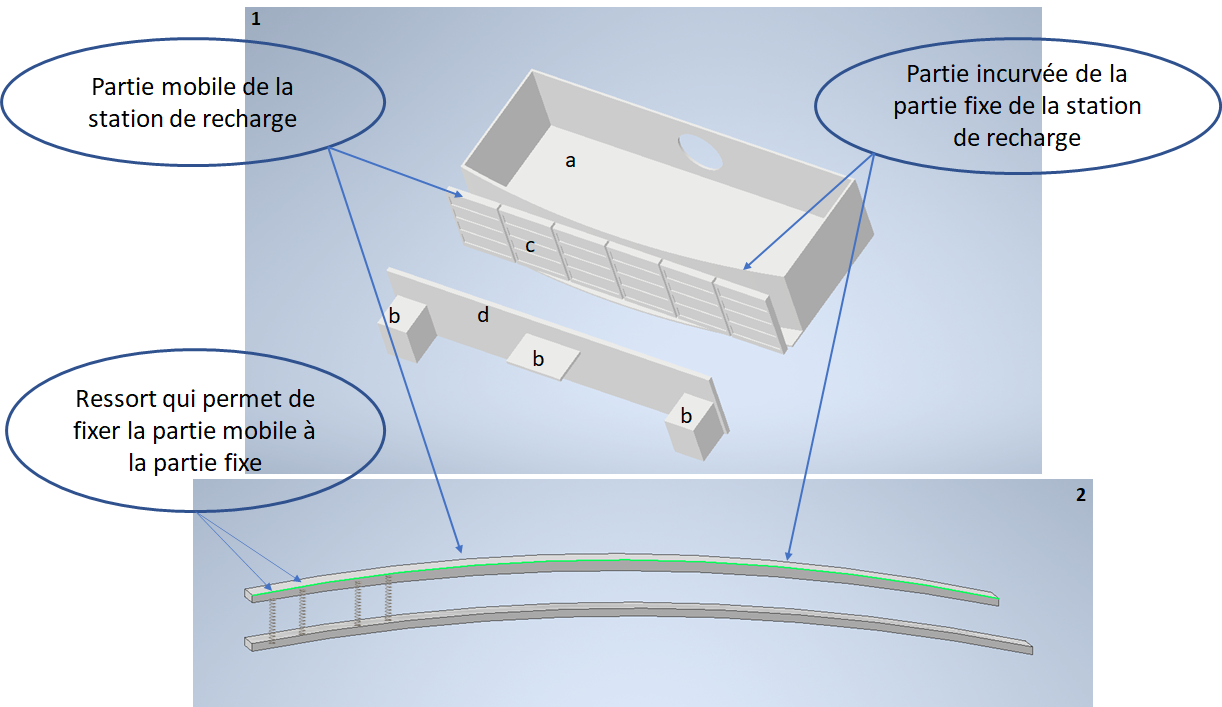
\includegraphics[scale=0.6]{images/station de recharge/fonctionnement station de rehcrage.png}
    \caption{Fonctionnement de la station de recharge en tenant compte des différentes caractéristiques}
    \label{fig:station de recharge}
\end{figure}
Élément de compréhension de la \textit{Figure 1} : Sur l’image \texttt{1} il faut imaginer que lorsque le robot n’est pas en contact avec la station de recharge les parties mobiles de celle-ci reviennent à leur place initiale et forment, comme l’image \texttt{2} le montre, un arc de cercle de même rayon de courbure que la partie fixe.\\

Une fois la conception 3D effectuée, nous avons dû choisir les procédés de fabrication pour chaque pièce. Après consultation des professeurs du \textit{pôle mécanique de l'ENSTA Bretagne}, nous avons convenu que la partie fixe de la station de recharge, qui contient une face incurvée \testit{(élément a)}, ainsi que les éléments rectangulaires permettant l'accroche de la partie contacteur sur le robot \testit{(éléments b)} seraient imprimés en 3D. Tandis que les parties mobiles de la station de recharge \testit{(éléments c)} et la partie contacteur du robot \testit{(éléments d)} seraient, elles, usinées dans du PVC afin de gagner du temps, d'obtenir des pièces plus rigides et également de réduire les coûts de fabrication. \\

Pour réaliser les contacteurs, nous avons choisi un plat d'aluminium brut afin de faire circuler le courant à travers. Ce plat de largeur 1cm et d'épaisseur 2mm s'insèrera dans les encoches prévues pour les contacteurs du robot et de la station de recharge. Les tests de conductivité n'ont pas pu être effectués à cause du contexte général sanitaire cependant il paraît important de pouvoir vérifier que la puissance émise par la station de recharge puisse être acheminée jusqu'à la batterie sur le robot. \\

Afin de mieux visualiser la station de recharge, des figures sont à retrouver en \hyperlink{annexe}{Annexe 2}.\\

\subsection{Partie Électronique}
Le deuxième partie importante se trouve être la partie électronique et électrique de la station de recharge. En effet après avoir réussi l'aspect mécanique du contact entre le robot et sa borne de recharge, nous avons dû réfléchir sur la façon de recharger la batterie \textit{LiPo}, ainsi que de transmettre une puissance nécessaire afin de recharger rapidement le robot et ainsi satisfaire les exigences. \\

Le fait d'utiliser une batterie \textit{LiPo}, complexifie légèrement l'approche de la recharge. En effet dans les chargeurs classiques \textit{LiPo}, il y a un contrôleur qui vérifie et permet la recharge des différentes cellules de la batterie de façon à ne pas les abîmer mais également de façon à ce que chaque cellule soit chargée correctement. Ce type de chargeur "\textit{intelligent}" nécessite une action humaine qui devait être substituée dans notre cas.\\
Après recherche de l'existant, nous avons rencontré un composant électronique qui permettait justement de contrôler la charge. Son nom : BMS pour \text{Battery Management System}. Ce composant surveille l'état de différents éléments de la batterie, tels que : \begin{itemize}[label=\textbullet, font=\small\color{blue}]
    \item la tension;
    \item la température;
    \item l'état de charge;
    \item ou encore le courant dans la batterie.
\end{itemize}
\\


Ce BMS s'insère entre l'alimentation qui servira à charger la batterie, et la batterie elle-même. Cependant il ne peut pas être inséré comme cela. En effet nous avons choisi un transformateur de type \textit{ordinateur} afin de délivrer une puissance permettant une charge rapide. Cependant ce transformateur délivre une tension de \textit{19,5V} et le BMS nécessite une alimentation de \textit{12,6V}. Il a donc fallu rajouter un \textit{hacheur série} permettant de convertir la tension alimentant le BMS. Afin d'illustrer de façon plus parlante cette architecture électronique, voici une figure illustrant cela :
\begin{figure}[H]
    \centering
    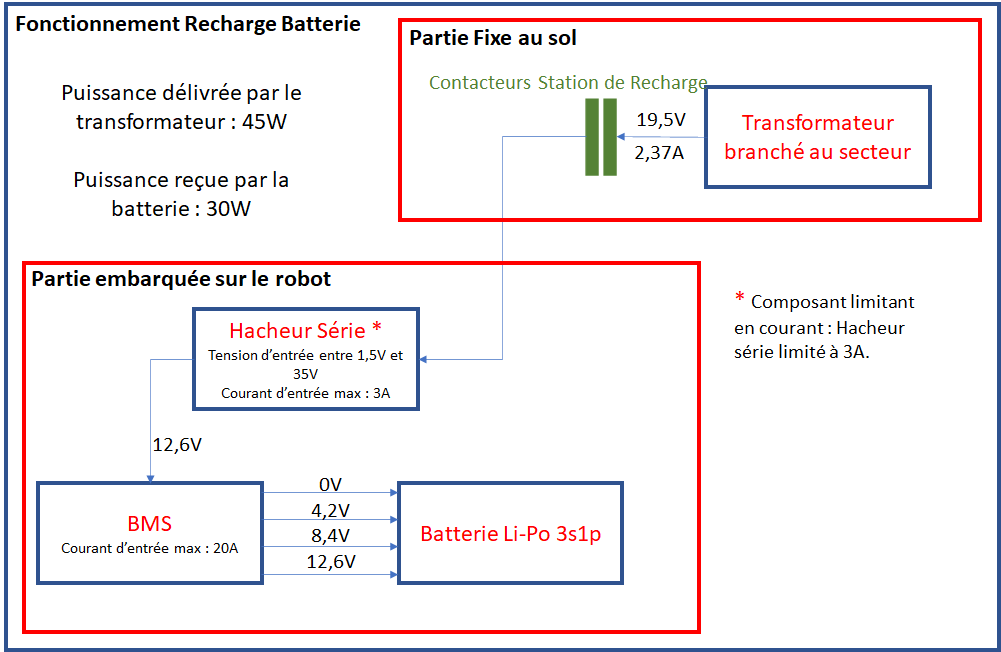
\includegraphics[scale=0.75]{images/station de recharge/Archi 2.png}
    \caption{Architecture Électronique}
    \label{fig:archi elec}
\end{figure}

Ces composants permettent une charge de la batterie à \textit{30W} ce qui est suffisant pour un prototype. Afin d'augmenter la puissance de charge il est nécessaire d'identifier le composant limitant qui est ici le \textit{hacheur série} (voir figure ci-dessus). En effet cet élément n'accepte pas un courant supérieur à 3A. Si l'on souhaite donc augmenter la vitesse de recharge il faudra changer ce composant qui a été choisi à la fois pour sa disponibilité et pour son coût relativement faible.\\

Enfin une remarque importante se situe autour de la nécessité d'alimenter le BMS en \textit{12,6V}. En effet nous n'avons trouvé aucune documentation en ligne sur le BMS dont nous avions besoin afin de charger une LiPo 3S. La seule indication qui nous a poussés à utiliser un \textit{hacheur série} se trouve dans une vidéo YouTube montrant la recharge d'une batterie avec le BMS en question (lien \href{https://www.youtube.com/watch?v=ySXtBuawf70}{ici}). Dans une continuité de projet, il serait intéressant de tester avec et sans le \textit{hacheur série}, au vue du faible coût de ce BMS. Un tel test serait intéressant afin de choisir un transformateur délivrant un courant supérieur, afin d'augmenter la puissance reçue par la batterie et ainsi de diminuer le temps de charge.

\subsection{Partie Informatique}
Nous allons maintenant traiter la partie informatique de la Station de Recharge. En effet bien que la charge soit autonome et ne nécessite pas de programmation particulière, le robot doit recevoir les informations suivantes : \begin{itemize}[label=\textbullet, font=\small\color{blue}]
    \item si le robot est bien en contact avec la station de recharge;
    \item l'état de charge de la batterie.
\end{itemize}

Pour réaliser cela, voici un schéma mettant en évidence les composants nécessaires : 
\begin{figure}[H]
    \centering
    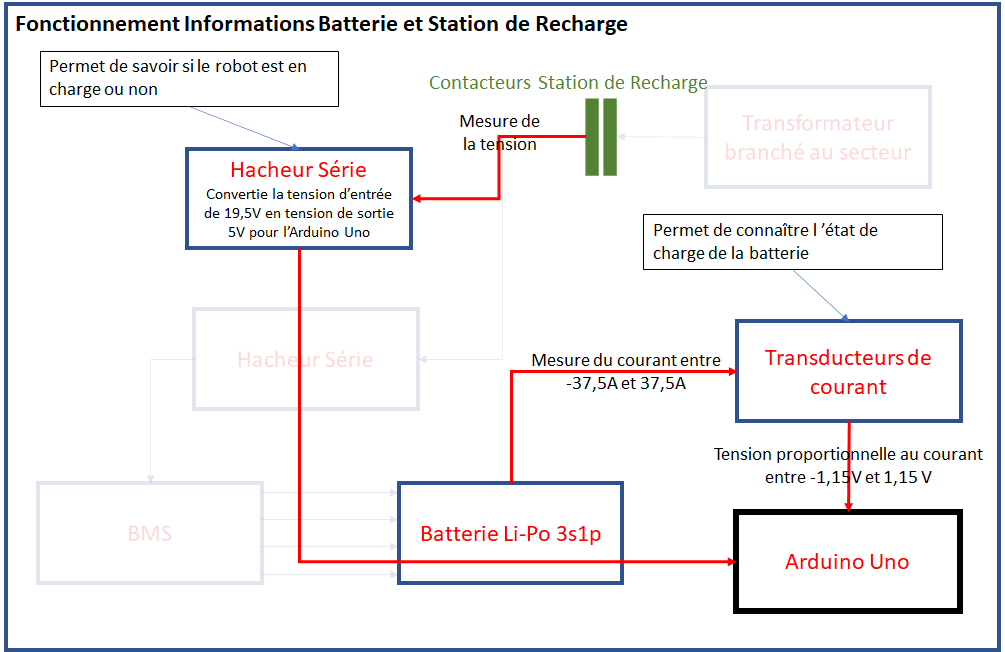
\includegraphics[scale=0.75]{images/station de recharge/Archi 3.png}
    \caption{Manières d'obtenir les informations importantes pour le robot}
    \label{fig:archi capteur}
\end{figure}

Ce schéma illustre les deux composants nécessaires à la prise d'information :\begin{itemize}[label=\textbullet, font=\small\color{blue}]
    \item D'une part un hacheur série connecté à un pin de l'Arduino Uno qui permet de savoir si de la tension passe le long des contacteurs de la partie robot. Cela permet de savoir si le contact avec la station de recharge est fait ou non.
    \item D'autre part un transducteur de courant qui mesure la courant circulant au sein de la batterie et qui renvoie comme information, une tension proportionnelle à l'intensité mesurée, sur un pin de l'Arduino Uno .
\end{itemize}
Il ne restera plus qu'à fournir un code Arduino qui renverra par topics ROS ces informations.


\subsection{État d'avancement de la station de recharge} \label{station}
Nous allons maintenant faire un point sur l'avancement  de la Station de Recharge qui était une partie attendue par Monsieur \textsc{chodorowski}. Vous pouvez retrouver la liste des composants en \hyperlink{annexe3}{Annexe 3}.\\

D'un point de vue mécanique, la station de recharge est opérationnelle sur le papier. Il reste : \begin{itemize}[label=\textbullet, font=\small\color{blue}]
    \item à tester la conductivité des contacteurs;
    \item à voir comment accrocher de façon simple, les ressorts qui permettent la liaison entre la partie mobile et la partie fixe de la Station de Recharge;
\end{itemize} 
Un premier test avait été effectué en laissant délibérément des petites encoches carrées dans les petites pièces rectangulaires mobile, et cela tenait. Nous n'avons pas pu tester l'accroche sur la partie fixe incurvée.\\

Pour la partie électronique, du fait de la séparation des alimentations moteur et contrôleur, le système et les composants mis en place devront être dupliqués afin que chaque batterie ait son propre BMS associé. Cela ne modifie en rien les contacteurs qui resteront les mêmes, il faudra cependant envisager de choisir un \textit{transformateur} délivrant un courant plus important, et donc envisager de changer de \testit{hacheur série}.\\

Enfin, du côté informatique, il ne restera plus qu'à fournir un code Arduino qui renverra par topics ROS ces informations. Cela ne pouvait se faire qu'en ayant les composants en main propre.

\pagebreak
\section{Intégration des composants}
Dans cette partie nous aborderons le thème de l'intégration des différents composants avec le middleware ROS.


\subsection{Encodeur}
\subsubsection{Procédure générale}
Tout d'abord nous allons aborder l'aspect intégration sous ROS des \textit{moteurs et encodeurs} et la commande des moteurs via topic ROS.\\

Tout d'abord, cette partie a été effectuée entièrement à distance, et l'ensemble de la commandabilité et contrôlabilité du robot n'a pu être faite. Les composants que nous disposions durant le confinement sont : \begin{itemize}[label=\textbullet, font=\small\color{blue}]
    \item L'ensemble carte Arduino UNO + Motor Shield,
    \item Un moteur et son encodeur,
    \item Une batterie LiPo.
\end{itemize}

Dans ce cadre limité, nous avons redéfini des objectifs atteignables qui sont : de réussir à s'abonner à un topic ROS émit par le NUC qui envoie la commande moteur, et de publier via l'Arduino un topic contenant le nombre de \textit{ticks} de l'encodeur.\\

Une fois cette mise au point faite, nous avons commencé par faire fonctionner le moteur et lire les valeurs de l'encodeur uniquement en utilisant un code Arduino. Cela nous a offert une meilleure compréhension du fonctionnement de ces composants. Afin de commander le moteur nous avons utilisé une librairie qui se nomme : "DualVNH5019MotorShield". Son installation sur Arduino est expliquée dans \href{https://github.com/AntoninLize/Projet_OrangeLabs/tree/master/Code/Arduino}{le README de ce lien}.\\

Le code Arduino qui permet uniquement de lire la valeur des encodeurs se trouve
\href{https://github.com/AntoninLize/Projet_OrangeLabs/tree/master/Code/Arduino/Encoder}{ici}.\\

Une fois avoir maîtrisé les commandes Arduino pour le moteur et l'encodeur, nous sommes passés sur la partie intégration sous ROS.\\

Pour cela nous avons dû installer ROS sur Arduino. Nous avons donc suivi \href{http://wiki.ros.org/rosserial_arduino/Tutorials/Arduino%20IDE%20Setup}{cette procédure} en remplaçant la version de ROS indigo par la version du ROS utilisé. Pour nous ce fut le ROS Melodic. En suivant toutes ces instructions et en relançant Arduino, dans les exemples nous pouvons retrouver des exemples de ROS sous Arduino.\\ 


Pour lancer le programme il faut se référer au README du dossier PubSub. Une fois les instructions suivies le programme fonctionne et le moteur se lance avec la commande donner dans le code C++ "Talker.cpp".\\

Les explications de code et les problèmes rencontrés au moment de la programmation, sont à retrouver en Annexe 4 page \pageref{annexe4}.\\


\subsubsection{État d'avancement de l'intégration des Encodeurs}
L'intégration des Encodeurs sous ROS est presque terminée. Il reste à modifier les types de message dans lesquels nous publions les informations. Cela sera relativement rapide si Arduino accepte le type de message en question.\\

Également nous n'avons pas eu, ni le temps ni les moyens d'effectuer le code permettant le contrôle du robot. Ainsi il reste à développer une régulation du robot en fonction de sa vitesse, de la trajectoire souhaitée, des obstacles détectés par le Lidar et enfin en fonction des erreurs corrigées par le PID.

\subsection{Caméra Realsense}
Pour la caméra realsense T265 que nous utilisons, il existe déjà un module ROS permettant la publication de tout les topics que nous utilisons. Ici, le  \href{https://github.com/IntelRealSense/realsense-ros}{lien} pour l’installation du SDK. \\


\begin{figure}[H]
    \centering
    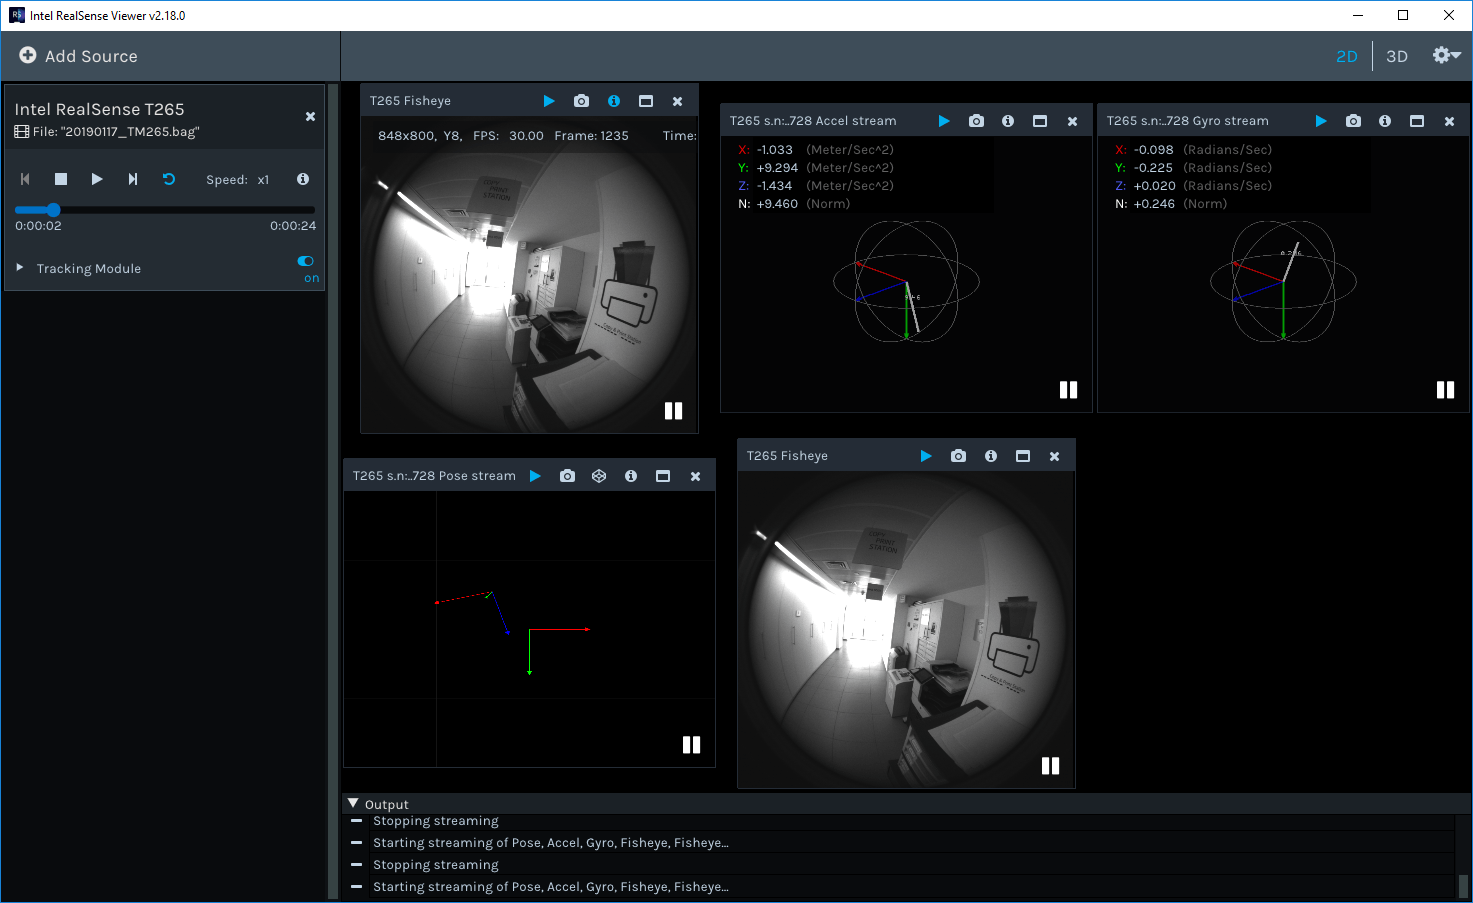
\includegraphics[scale=0.25]{images/robot/realsense-viewer.png}
    \caption{Outil de visualisation pour la caméra Realsense}
    \label{fig:archi elec}
\end{figure}
Une fois ce module installé, il suffit de lancer les nodes avec la commande : \\
\textbf{roslaunch realsense2-camera rs-camera.launch} \\

Les topics publiés qui sont intéressants pour notre projet sont : \begin{itemize}[label=\textbullet, font=\small\color{blue}]
    \item Les topics image brute,
    \item Le topic IMU,
    \item Le topic odométrie. 
\end{itemize}



\subsection{RP Lidar}
Le LIDAR que nous utilisons est un RPLIDAR A2 de chez Slamtech, l'ensemble des SDK nécessaires à l'utilisation de ce LIDAR sont fournis par le constructeur(lien \href{https://www.slamtec.com/en/Support#rplidar-a-series}{ici}) \\

Pour l'installation, il faut tout d'abord installer le module permettant de faire fonctionner le LIDAR puis le module permettant le lancement avec ROS (et donc la visualisation avec RVIZ). Une fois ces packages installés, on peut utiliser le LIDAR et avoir accès au topic classique \textbf{scan}. \\
\\


\begin{figure}[h]
\centering
\begin{minipage}[b]{.5\textwidth}
  \centering
  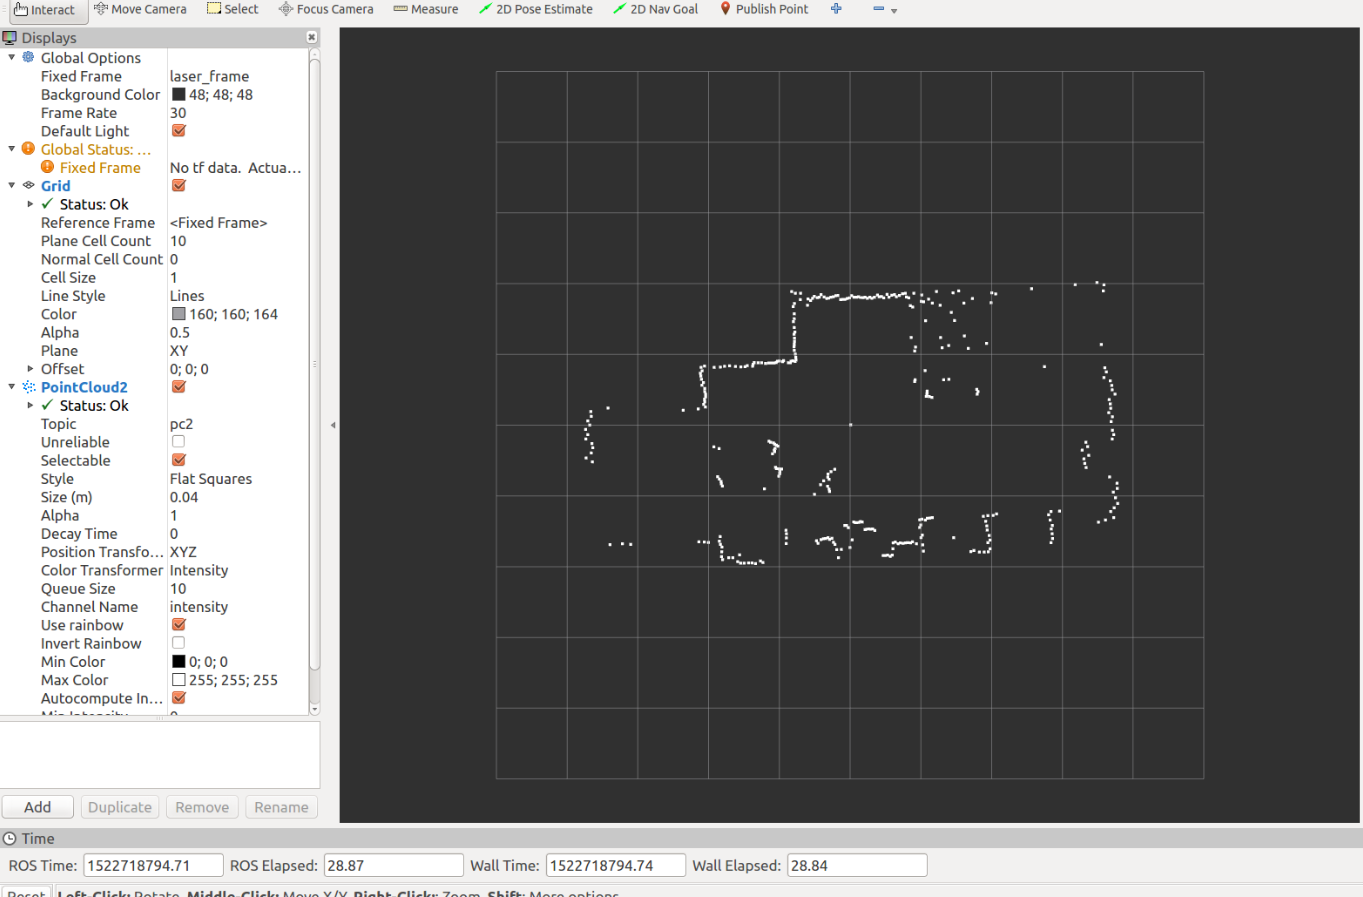
\includegraphics[width=.95\linewidth]{images/robot/lidar.png}
  \captionof*{figure}{a) Détection des points}
  \label{fig:archi elec}
\end{minipage}%
%
% Second graph
\begin{minipage}[b]{.61\textwidth}
  \centering
  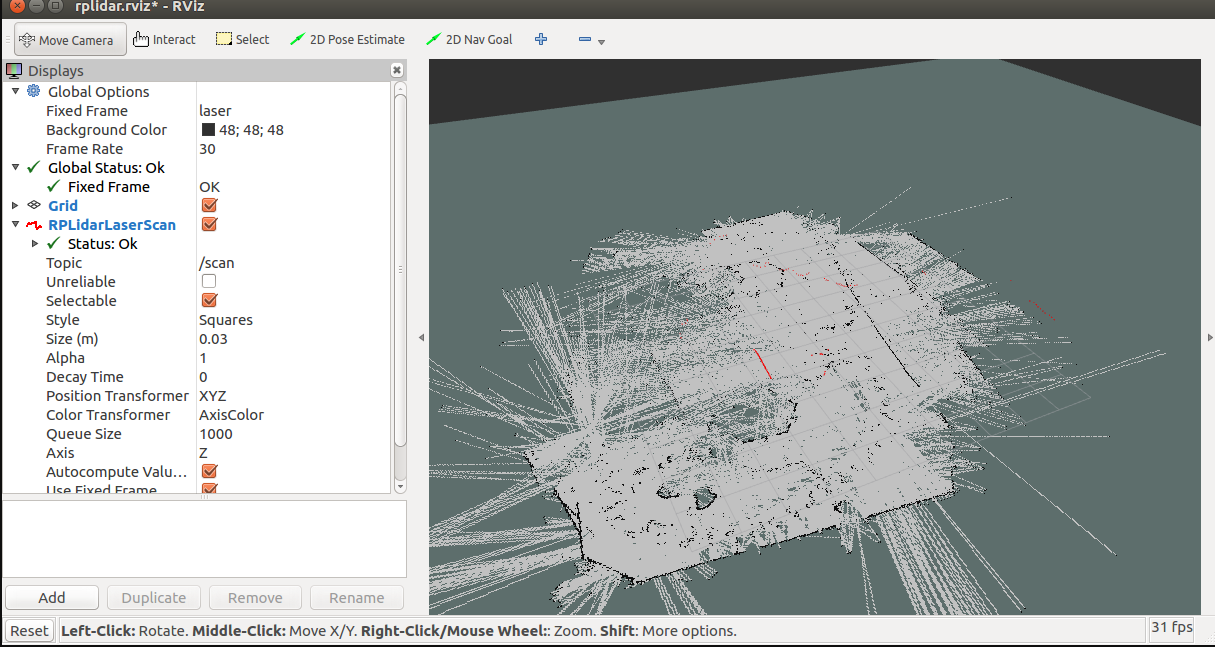
\includegraphics[width=.95\linewidth]{images/robot/lidarslam.png}
  \captionof*{figure}{b) Application du SLAM}
  \label{fig:archi elec}
\end{minipage}
%


\vspace{3mm}
\caption{Visualisation avec RVIZ}
\label{fig:archi elec}
\end{figure}


Touts les fichiers contenant les drivers sont à retrouver sur le Git du projet. Le node-graph est, quant à lui, à retrouver en page \pageref{annexe5}.

\section{Résultats et continuité}
Dans cette ultime partie, nous allons traiter des résultats et de l'avancement général du projet. Nous parlerons également des possibilités de suite et de la continuité des différentes tâches. Pour cela, nous allons diviser la suite en deux paragraphes : le premier pour parler du robot et le second pour la station de recharge.\\

Concernant le robot, l'installation sur le robot des capteurs tels que le Lidar ou la caméra Realsens n'ont pas pu être fait puisque nous n'avions plus le robot sous la main depuis début Mars. Concernant les intégrations sous ROS du NUC, du Lidar et de la caméra, elles sont opérationnelles et ne nécessitent qu'un code qui gère la navigation. L'alimentation a été traité antérieurement, elle devra être tout de même testée en situation réelle. Le mât a été délibérément abandonné dans le contexte actuel mais avec une éventuelle reprise de projet, ceci redeviendra un critère important. Concernant le châssis, celui-ci permet d'accueillir tous les capteurs et installations souhaités. Les intégrations des moteurs et encodeurs a été effectuées. Il reste cependant à coder un programme permettant de contrôler la vitesse et la trajectoire du robot.\\

Concernant la station de recharge, nous n'allons pas nous attarder dessus. Vous pouvez retrouver page \pageref{station} l'état d'avancement de la station, les tâches à réaliser et les possibles améliorations envisagées. Pour résumer, toute la partie théorique a été effectuée. Il reste l'aspect pratique et le test des solutions envisagées.



\section{Conclusion}

Afin de conclure ce rapport mais également ce projet, nous tenions à remercier de nouveau Monsieur CHODOROWSKI qui nous a donné l'opportunité et les moyens de travailler sur ce beau défi. \\

Les premiers objectifs fixés ont, certes, été revus à la baisse, néanmoins les leçons apprises tout au long de ce travail sont très nombreuses. Nous n'allons pas dresser la liste de chacune, cependant au delà de l'aspect théorique et pratique en robotique, nous avons acquis tout au long de ce projet des compétences de gestion et de suivi de projet. Les rencontres et les discussions hebdomadaires avec notre encadrant, les libertés de décisions qu'il nous a offertes, la répartition du travail entre nous, tout ceci nous a permis de mieux découvrir le travail d'un ingénieur en relation avec une entreprise commanditaire d'un robot. \\

Ce projet professionnalisant nous servira à coup sûr dans nos expériences futures, que ce soit en stage ou dans notre futur métier. \\

Pour conclure, notre travail de présentation, d'explication et de synthèse a pour vocation la continuité de ce projet. Nous espérons qu'avec toutes nos recherches et nos travaux, ce projet ambitieux pourra arriver à son terme. Nous sommes heureux d'avoir pu y ajouter notre contribution.

\pagebreak
\listoffigures

\pagebreak
\section{Annexe}
\subsection{Annexe 1 : Liste matériel pour le robot}

\begin{figure}[H]
     \centering
     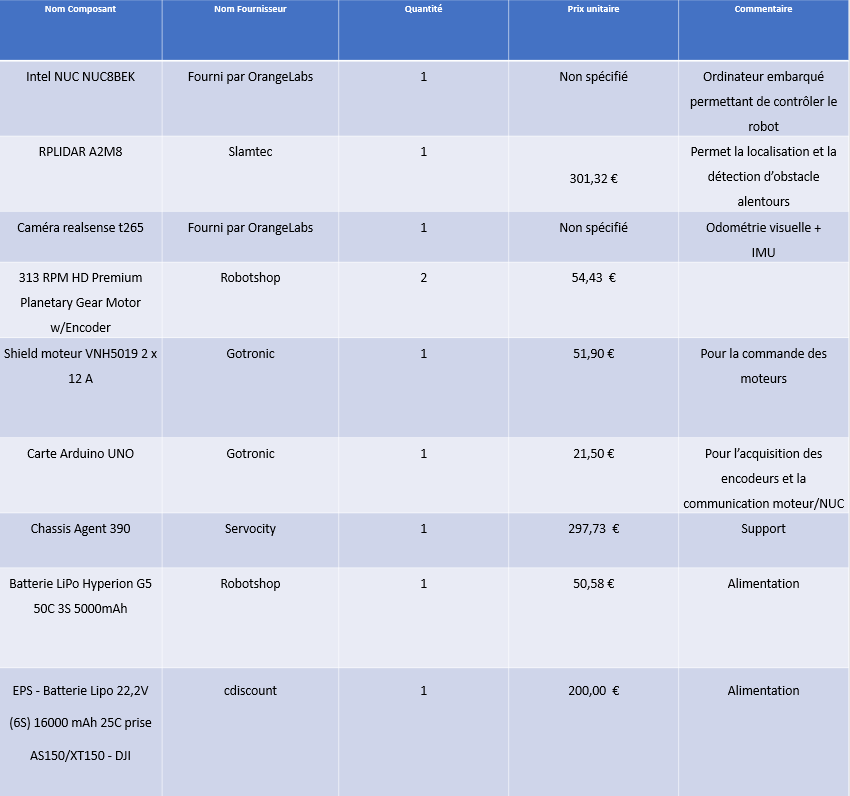
\includegraphics[scale=0.7]{images/robot/liste_composants_robot.png}
     \caption{Liste matériel pour le robot}
     \label{matos}
\end{figure}

\subsection{Annexe 2 : Complément Modélisation Station de Recharge}
\hypertarget{annexe}
Les modélisations suivantes permettent une meilleur compréhension de la partie mécanique de la station de recharge. \
\begin{figure}[H]
     \centering
     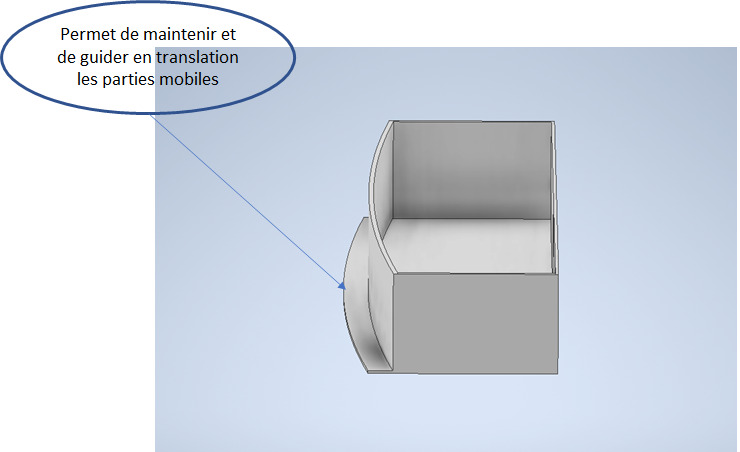
\includegraphics[scale=1]{images/station de recharge/partie fixe station.png}
     \caption{Partie Fixe Station de Recharge}
     \label{fig:station de recharge}
\end{figure}

\begin{figure}[H]
     \centering
     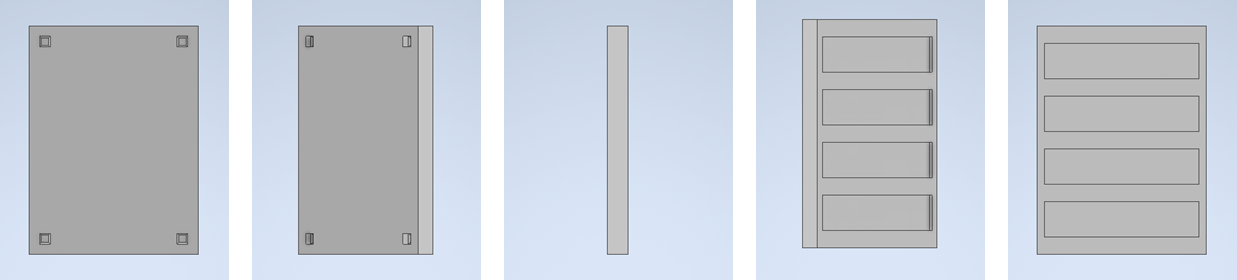
\includegraphics[scale=0.6]{images/station de recharge/partie mobile station.png}
     \caption{Partie Mobile Station de Recharge}
     \label{fig:station de recharge}
\end{figure}

\begin{figure}[H]
     \centering
     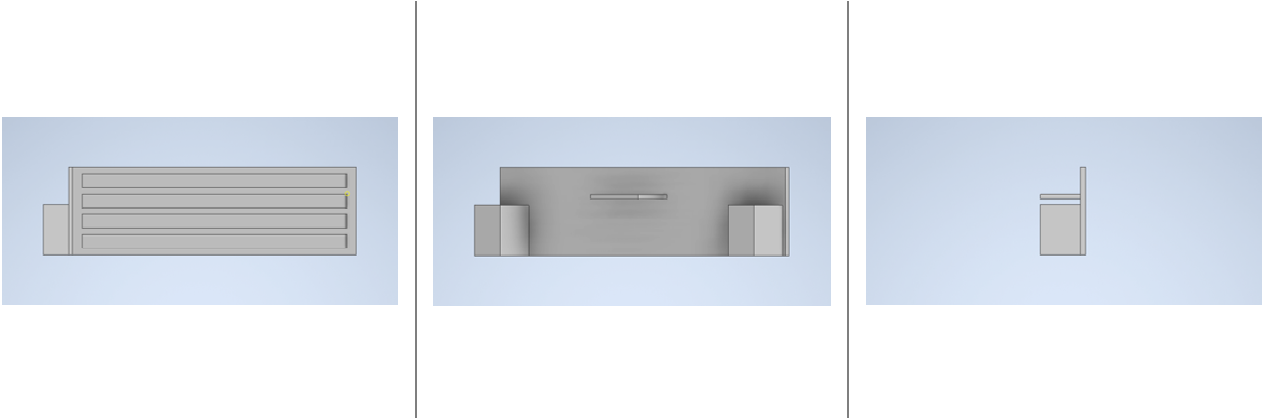
\includegraphics[scale=0.6]{images/station de recharge/partie fixe robot.png}
     \caption{Partie Fixe Robot}
     \label{fig:station de recharge}
\end{figure}

\begin{figure}[H]
     \centering
     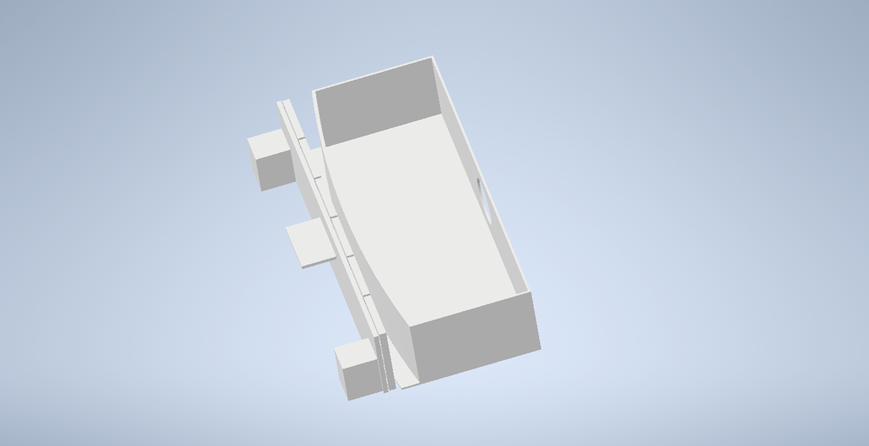
\includegraphics[scale=0.8]{images/station de recharge/contact station.png}
     \caption{Contact Robot + Station de Recharge}
     \label{fig:station de recharge}
\end{figure}

\begin{figure}[H]
     \centering
     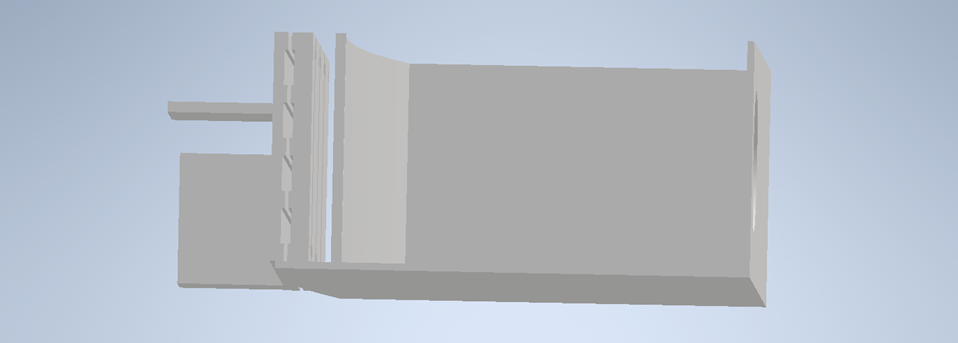
\includegraphics[scale=0.8]{images/station de recharge/contact station de profil.png}
     \caption{Contact Robot + Station de Recharge de profil}
     \label{fig:station de recharge}
\end{figure}

\subsection{Annexe 3 : Liste matériel pour la station de recharge}
\hypertarget{annexe3}

\begin{figure}[H]
     \centering
     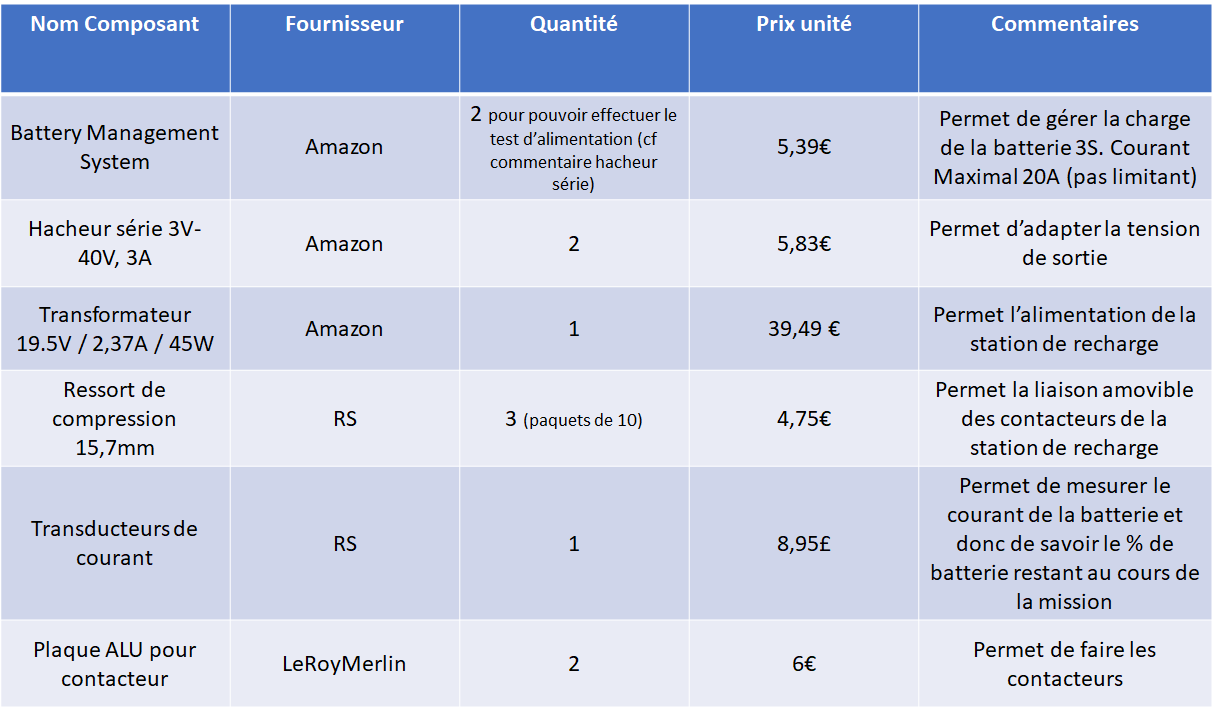
\includegraphics[scale=0.6]{images/station de recharge/liste matos.png}
     \caption{Liste matériel pour la station de recharge}
     \label{matos}
\end{figure}


\subsection{Annexe 4 : Tutoriel codes Encodeurs et Moteurs} \label{annexe4}
\subsubsection{Explication des codes}

Le code Arduino qui permet de commander le moteur en envoyant une commande entre -400 et 400 via les fonctions \textit{setM1Speed} et \textit{setM2Speed} (dans le cas où il y a deux moteurs) se trouve \href{https://github.com/AntoninLize/Projet_OrangeLabs/tree/master/Code/Arduino/Commande_moteur}{ici}. Le code a été écrit de telle sorte à pouvoir piloter les moteurs via le clavier numérique : \begin{itemize}[label=\textbullet, font=\small\color{blue}]
    \item "8" pour avancer,
    \item "5" pour s'arrêter,
    \item "2" pour reculer.
\end{itemize}\\

C'est à partir de l'exemple \textit{pubsub} que nous avons construit le code permettant de lire la commande sur un topic et de publier sur un autre les valeurs encodeurs. Pour le code \href{https://github.com/AntoninLize/Projet_OrangeLabs/tree/master/Code/Arduino/pubsub}{suivre ce lien}. Le code en lui même est relativement simple, cependant le ROS sous Arduino est très légèrement différent que sous C++ et quelques problèmes sont apparus comme par exemple le fait de devoir utiliser un \textit{char *} afin de récupérer les valeurs de commandes moteurs.\\

Pour le moment le code ne reçoit et n'envoie que des topics de type String, dans les besoins du projet il faudra utiliser des messages déjà implémentés comme par exemple un message de type \href{http://docs.ros.org/api/geometry_msgs/html/msg/Twist.html}{Twist}.\\

Enfin afin de publier les topics de commande, nous avons implémenté un code que l'on peut retrouver dans un workspace ROS sur notre GitHub. Les codes sont dans le dossier /src qui contient deux codes en C++ : 
\begin{itemize}[label=\textbullet, font=\small\color{blue}]
    \item Talker.cpp qui permet de publier sur un topic ROS nommé \textit{cmd motor} la commande moteur,
    \item PID.cpp qui est un exemple de PID utilisé sur un autre projet et qui pourra être réadapté pour ce projet.
\end{itemize}\\

\subsubsection{Problèmes rencontrés}

L'un des principaux problème fut au moment de publier la valeur de l'encodeur. En effet avec les premières versions nous pouvions lire sur le topic "value encoder" des valeurs qui ne correspondaient pas aux valeurs attendues. En effet nous avions environ 50 ticks par tour alors que la documentation moteur indiquait 322 ticks par tour et que nous avions déjà testé l'encodeur uniquement avec Arduino et les valeurs étaient cohérentes.\\ 

Après recherche nous avons réalisé que la fréquence à laquelle nous parcourions la boucle loop() du programme Arduino n'était pas suffisante par rapport à la fréquence de rotation du moteur. Autrement dit, nous ne lisions qu'une valeur encodeur sur six. Pour comprendre d'où venait le problème, nous avons dû regarder combien de cycles d'horloge durait chaque commande dans le loop(). Les résultats de ces tests sont en commentaires du programme Arduino "pubsub.ino". Nous avons constaté que ce qui prenait le plus de temps était la conversion en \textit{char *} ainsi que la publication du topic \textit{"value encoder"} et de la commande "\textit{spinOnce()}.\\

Afin d'y remédier, nous avons choisi de ne publier la valeur du topic \textit{"value encoder"} que toutes les 100 passages de boucle loop(). Ceci nous a permis de pouvoir lire la valeur encodeur à chaque loop() de façon plus rapide et ainsi éviter de sauter des valeurs encodeurs, tout en publiant assez régulièrement afin d'afficher tous les changements de ticks.

\subsection{Annexe 5 : Node graph } \label{annexe5}


\begin{figure}[H]
    \centering
    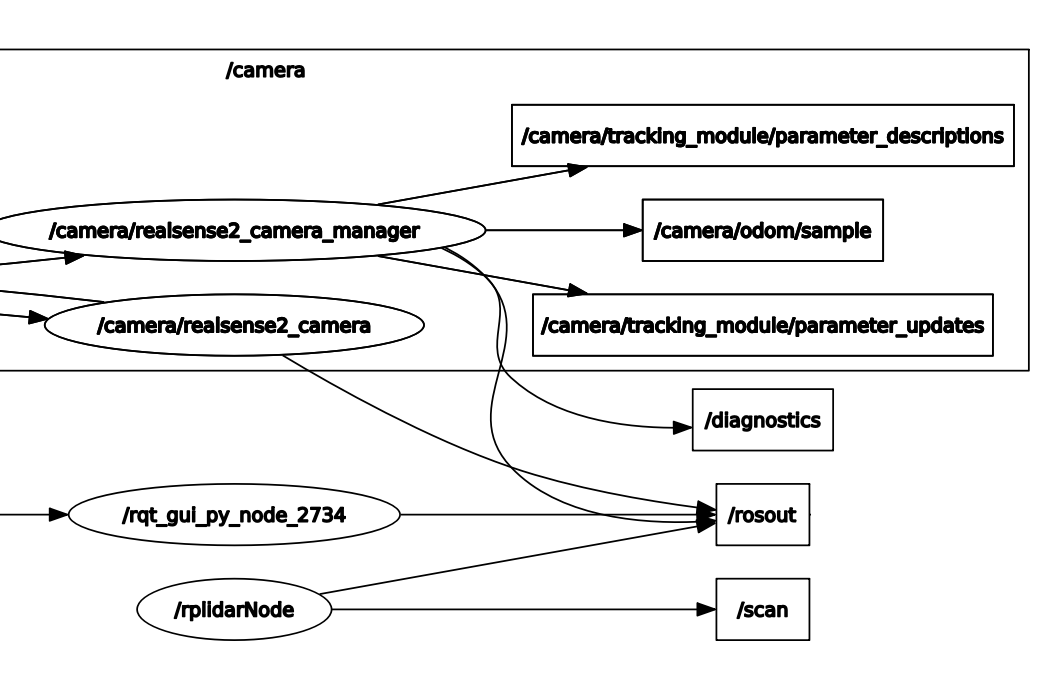
\includegraphics[width = 15cm,height = 10cm]{images/robot/node_graph.png}
    \caption{Node Graph : LIDAR et Realsense}
    \label{fig:archi elec}
\end{figure}

\end{document} 